
\documentclass[a4paper,8pt]{article}
\usepackage{graphicx}
\usepackage[margin=0.5in,top=0.5in,bottom=0.5in,left=0.75in]{geometry}
\usepackage{fancyhdr} % for custom headers and footers
\pagestyle{fancy} % set page style to fancy
\renewcommand{\headrulewidth}{0pt}
\fancyhf{} % clear default header and footer
\fancyfoot[C]{\thepage} % set center of footer to be the page number
\usepackage{float}
\usepackage{makeidx}

\makeindex

\title{DIP Assignments}
\begin{document}
\maketitle
\centering
M.Sc. Computer Science, 3rd Sem, 2022-23


Registration No. : 017171 of 22017-2018


Roll: 90/MCS NO.210010


Session: 2021-2023


Paper Code: MCS-DSE-312
\clearpage
\tableofcontents
\clearpage
        \section{Histogram Find}
        \begin{verbatim}
        from PIL import Image
from PIL import ImageDraw

# Open image and get pixel values
img = Image.open('input1.jpg')
img = img.convert('L')
pixels = list(img.getdata())

# Create histogram
histogram = [0] * 256
for pixel in pixels:
    print(pixel)
    histogram[pixel] += 1

# Normalize histogram values to [0, 255]
max_count = max(histogram)
normalized_hist = [round((count / max_count) * 255) for count in histogram]

# Create histogram image
hist_img = Image.new('RGB', (256, 256), color='white')
draw = ImageDraw.Draw(hist_img)
for i, count in enumerate(normalized_hist):
    draw.line((i, 255, i, 255-count), fill='black', width=1)

# Save histogram image
hist_img.save('histogram.png')


        \end{verbatim}
        
        \begin{figure}[H]
        \centering
        \begin{minipage}{0.4\linewidth}
        \centering
        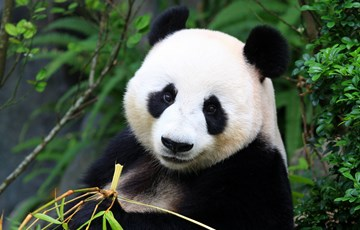
\includegraphics[width=\linewidth]{output/input1.jpg}
        \caption{Input}
        \end{minipage}
        \hfill
        \begin{minipage}{0.4\linewidth}
        \centering
        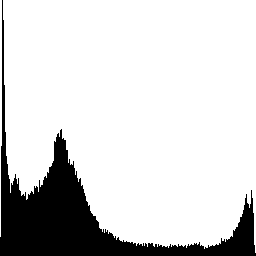
\includegraphics[width=\linewidth]{output/Histogram Find_output.png}
        \caption{Output}
        \end{minipage}
        \end{figure}
        \clearpage
        
        \section{Histogram Equalization}
        \begin{verbatim}
        import sys

input_file = sys.argv[1]
output_file = sys.argv[2]

with open(input_file, 'r') as picture:
    element = picture.readlines()

frequency = {}
pdf = {}
cdf = {}
mapping = {}
for i in range(256):
    frequency[f'{i}'] = 0
    pdf[f'{i}'] = 0
    cdf[f'{i}'] = 0
    mapping[f'{i}'] = 0
    
for i in range(4, len(element)-4):
    frequency[element[i].replace('\n', '')] += 1

for i in range(256):
    pdf[f'{i}'] = round(frequency[f'{i}'] / (len(element)-4), 3)

cdf['0'] = pdf['0']
for i in range(1, 256):
    cdf[f'{i}'] = cdf[f'{i-1}'] + pdf[f'{i}']

for i in range(256):
    mapping[f'{i}'] = round(255 * cdf[f'{i}'])

with open(output_file, 'w') as out:
    for i in range(4, len(element)-4):
        element[i] = str(mapping[element[i].replace('\n', '')]) + '\n'
    out.writelines(element)


        \end{verbatim}
        
        \begin{figure}[H]
        \centering
        \begin{minipage}{0.4\linewidth}
        \centering
        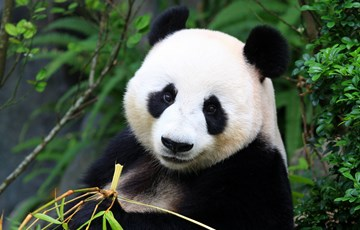
\includegraphics[width=\linewidth]{output/input1.jpg}
        \caption{Input}
        \end{minipage}
        \hfill
        \begin{minipage}{0.4\linewidth}
        \centering
        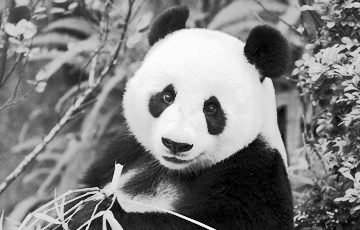
\includegraphics[width=\linewidth]{output/Histogram Equalization_output.png}
        \caption{Output}
        \end{minipage}
        \end{figure}
        \clearpage
        
        \section{Log Transformation}
        \begin{verbatim}
        from math import log10
import sys
import numpy as np


input_file = sys.argv[1]
output_file = sys.argv[2]
input_image = np.loadtxt(input_file, skiprows=3)


with open(input_file, 'r') as picture:
    element = picture.readlines()

with open(output_file, 'w') as out:
    for i in range(len(element) - 4):
        element[i+4] = str( int(104 * log10(1 + int(element[i+4].replace('\n', ''))))) + '\n'
    out.writelines(element)

        \end{verbatim}
        
        \begin{figure}[H]
        \centering
        \begin{minipage}{0.4\linewidth}
        \centering
        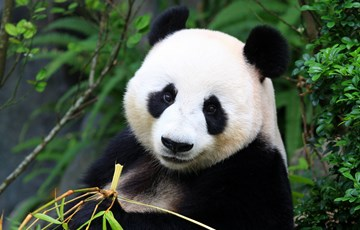
\includegraphics[width=\linewidth]{output/input1.jpg}
        \caption{Input}
        \end{minipage}
        \hfill
        \begin{minipage}{0.4\linewidth}
        \centering
        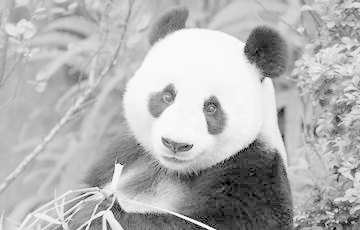
\includegraphics[width=\linewidth]{output/Log Transformation_output.png}
        \caption{Output}
        \end{minipage}
        \end{figure}
        \clearpage
        
        \section{Power Law Transformation}
        \begin{verbatim}
        import sys
from math import pow


input_file = sys.argv[1]
output_file = sys.argv[2]
gamma = 2
C = 1.3

with open(input_file, 'r') as picture:
    element = picture.readlines()

with open(output_file, 'w') as out:
    for i in range(len(element) - 4):
        pix = int(C * pow(int(element[i+4].replace('\n', '')), gamma))
        if pix > 255:
            element[i+4] = '255\n'
        elif pix < 0:
            element[i+4] = '0\n'
        else:
            element[i+4] = str(pix) + '\n'
    out.writelines(element)


        \end{verbatim}
        
        \begin{figure}[H]
        \centering
        \begin{minipage}{0.4\linewidth}
        \centering
        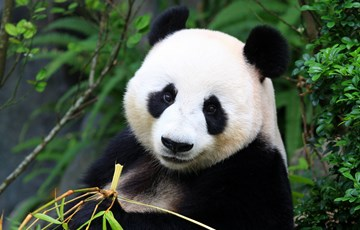
\includegraphics[width=\linewidth]{output/input1.jpg}
        \caption{Input}
        \end{minipage}
        \hfill
        \begin{minipage}{0.4\linewidth}
        \centering
        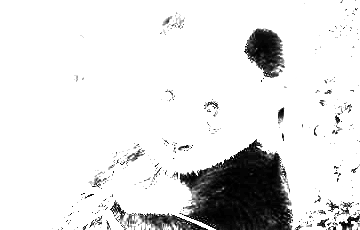
\includegraphics[width=\linewidth]{output/Power Law Transformation_output.png}
        \caption{Output}
        \end{minipage}
        \end{figure}
        \clearpage
        
        \section{Pixel Distance}
        \begin{verbatim}
        import sys
from math import sqrt

# Parse command-line arguments
print(sys.argv)
if len(sys.argv) != 7:
    print("Usage: python distances.py <input_file> <output_file> <x1> <y1> <x2> <y2>")
    sys.exit()

input_file = sys.argv[1]
output_file = sys.argv[2]
x1, y1, x2, y2 = int(sys.argv[3]),int(sys.argv[4]),int(sys.argv[5]),int(sys.argv[6])

# Read the input image file line by line
with open(input_file, 'r') as f:
    lines = f.readlines()

# Extract the image dimensions and pixel values
assert lines[0].startswith('P2')
width, height = map(int, lines[2].split())
max_value = int(lines[3])
pixels = [[int(val) for val in line.split()] for line in lines[4:]]

# Compute the Euclidean distance between the two pixels
euclidean_distance = sqrt((x1 - x2)**2 + (y1 - y2)**2)

# Compute the D4 distance between the two pixels
d4_distance = abs(x1 - x2) + abs(y1 - y2)

# Compute the D8 distance between the two pixels
d8_distance = max(abs(x1 - x2), abs(y1 - y2))

# Compute the Dm distance between the two pixels
dm_distance = max(abs(x1 - x2), abs(y1 - y2), abs(x1 - y1), abs(x2 - y2))

# Write the distances to the output file
with open(output_file, 'w') as f:
    f.write(f"Euclidean distance: {euclidean_distance:.2f}\n")
    f.write(f"D4 distance: {d4_distance}\n")
    f.write(f"D8 distance: {d8_distance}\n")
    f.write(f"Dm distance: {dm_distance}\n")


        \end{verbatim}
        
        \begin{figure}[H]
        \centering
        \begin{minipage}{0.4\linewidth}
        \centering
        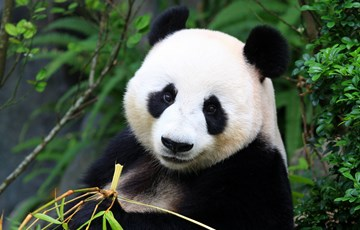
\includegraphics[width=\linewidth]{output/input1.jpg}
        \caption{Input}
        \end{minipage}
        \hfill
        \begin{minipage}{0.4\linewidth}
        \centering
        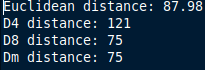
\includegraphics[width=\linewidth]{output/Pixel Distance_output.png}
        \caption{Output}
        \end{minipage}
        \end{figure}
        \clearpage
        
        \section{Min Filter}
        \begin{verbatim}
        import numpy as np
import sys

input_image = sys.argv[1]
with open(input_image, 'r') as picture:
    element = picture.readlines()

def avg_filter(pixel, start, filter_size):
    new_pixel = np.zeros((pixel.shape[0],pixel.shape[1]))
    for i in range(start, pixel.shape[0]-start):
        for j in range(start, pixel.shape[1]-start):
            new_pixel[i][j] = int(pixel[i-start:i+filter_size-start, j-start:j+filter_size-start].min())

    return new_pixel

filter_size = 3
row = int(element[2].replace('\n', '').split()[1])
col = int(element[2].replace('\n', '').split()[0])
pixel = np.zeros((row + filter_size - 1, col + filter_size - 1))
a = 4
start = (filter_size - 1)//2
for i in range(start, pixel.shape[0]-start):
    for j in range(start, pixel.shape[1]-start):
        pixel[i][j] = int(element[a].replace('\n', ''))
        a += 1

new_pixel = avg_filter(pixel, start, filter_size)
b = 4
for i in range(start, new_pixel.shape[0]-start):
        for j in range(start, new_pixel.shape[1]-start):
            element[b] = str(int(new_pixel[i][j]))+'\n'
            b += 1
name = sys.argv[2]
with open(name, 'w') as out:
    out.writelines(element)

        \end{verbatim}
        
        \begin{figure}[H]
        \centering
        \begin{minipage}{0.4\linewidth}
        \centering
        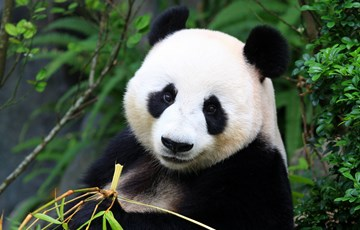
\includegraphics[width=\linewidth]{output/input1.jpg}
        \caption{Input}
        \end{minipage}
        \hfill
        \begin{minipage}{0.4\linewidth}
        \centering
        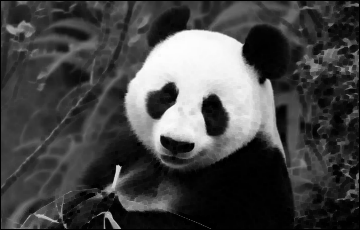
\includegraphics[width=\linewidth]{output/Min Filter_output.png}
        \caption{Output}
        \end{minipage}
        \end{figure}
        \clearpage
        
        \section{Constrst Streaching}
        \begin{verbatim}
        import sys

# read input file name and output file name from command line arguments
if len(sys.argv) < 3:
    print('Usage: python contrast.py <input_file> <output_file>')
    sys.exit(1)
input_file = sys.argv[1]
output_file = sys.argv[2]

# read pixel values from input file
with open(input_file, 'r') as picture:
    element = picture.readlines()

pixel = []
for i in range(len(element) - 4):
    pixel.append(int(element[i+4].replace('\n', '')))

# calculate maximum and minimum pixel values
max_pixel = max(pixel)
min_pixel = min(pixel)

# write updated pixel values to output file
with open(output_file, 'w') as out:
    for i in range(len(element) - 4):
        element[i+4] = str(round(((pixel[i] - min_pixel)/(max_pixel - min_pixel)*255), 0)) + '\n'
    out.writelines(element)


        \end{verbatim}
        
        \begin{figure}[H]
        \centering
        \begin{minipage}{0.4\linewidth}
        \centering
        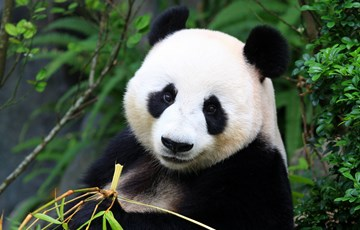
\includegraphics[width=\linewidth]{output/input1.jpg}
        \caption{Input}
        \end{minipage}
        \hfill
        \begin{minipage}{0.4\linewidth}
        \centering
        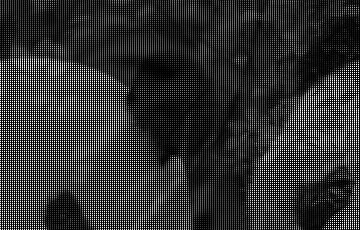
\includegraphics[width=\linewidth]{output/Constrst Streaching_output.png}
        \caption{Output}
        \end{minipage}
        \end{figure}
        \clearpage
        
        \section{Negative Transformation}
        \begin{verbatim}
        import sys

if len(sys.argv) < 3:
    print("Usage: python myscript.py input.pgm output.pgm")
    sys.exit(1)

input_file = sys.argv[1]
output_file = sys.argv[2]

with open(input_file, 'r') as picture:
    element = picture.readlines()

with open(output_file, 'w') as out:
    for i in range(len(element) - 4):
        element[i+4] = str(255 - int(element[i+4].replace('\n', ''))) + '\n'
    out.writelines(element)


        \end{verbatim}
        
        \begin{figure}[H]
        \centering
        \begin{minipage}{0.4\linewidth}
        \centering
        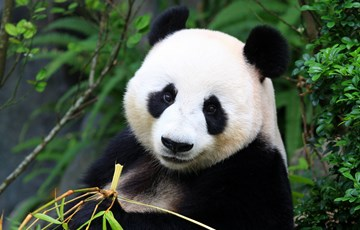
\includegraphics[width=\linewidth]{output/input1.jpg}
        \caption{Input}
        \end{minipage}
        \hfill
        \begin{minipage}{0.4\linewidth}
        \centering
        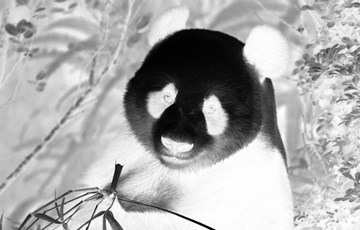
\includegraphics[width=\linewidth]{output/Negative Transformation_output.png}
        \caption{Output}
        \end{minipage}
        \end{figure}
        \clearpage
        
        \section{Max Filter}
        \begin{verbatim}
        import numpy as np
import sys

input_image = sys.argv[1]
with open(input_image, 'r') as picture:
    element = picture.readlines()

def avg_filter(pixel, start, filter_size):
    new_pixel = np.zeros((pixel.shape[0],pixel.shape[1]))
    for i in range(start, pixel.shape[0]-start):
        for j in range(start, pixel.shape[1]-start):
            new_pixel[i][j] = int(pixel[i-start:i+filter_size-start, j-start:j+filter_size-start].max())

    return new_pixel

filter_size = 3
row = int(element[2].replace('\n', '').split()[1])
col = int(element[2].replace('\n', '').split()[0])
pixel = np.zeros((row + filter_size - 1, col + filter_size - 1))
a = 4
start = (filter_size - 1)//2
for i in range(start, pixel.shape[0]-start):
    for j in range(start, pixel.shape[1]-start):
        pixel[i][j] = int(element[a].replace('\n', ''))
        a += 1

new_pixel = avg_filter(pixel, start, filter_size)
b = 4
for i in range(start, new_pixel.shape[0]-start):
        for j in range(start, new_pixel.shape[1]-start):
            element[b] = str(int(new_pixel[i][j]))+'\n'
            b += 1
name = sys.argv[2]
with open(name, 'w') as out:
    out.writelines(element)


        \end{verbatim}
        
        \begin{figure}[H]
        \centering
        \begin{minipage}{0.4\linewidth}
        \centering
        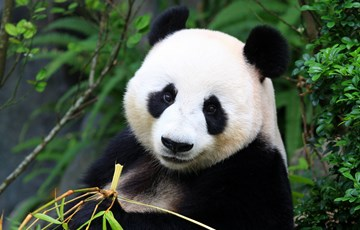
\includegraphics[width=\linewidth]{output/input1.jpg}
        \caption{Input}
        \end{minipage}
        \hfill
        \begin{minipage}{0.4\linewidth}
        \centering
        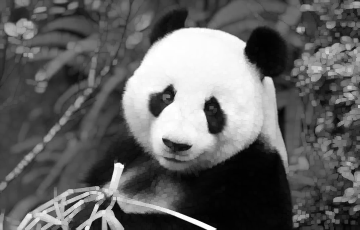
\includegraphics[width=\linewidth]{output/Max Filter_output.png}
        \caption{Output}
        \end{minipage}
        \end{figure}
        \clearpage
        
        \section{Average Filter}
        \begin{verbatim}
        import numpy as np

input_image = sys.argv[1]
with open(input_image, 'r') as picture:
    element = picture.readlines()

def avg_filter(pixel, start, filter_size):
    new_pixel = np.zeros((pixel.shape[0],pixel.shape[1]))
    for i in range(start, pixel.shape[0]-start):
        for j in range(start, pixel.shape[1]-start):
            new_pixel[i][j] = int(pixel[i-start:i+filter_size-start, j-start:j+filter_size-start].mean())

    return new_pixel

filter_size = 3
row = int(element[2].replace('\n', '').split()[1])
col = int(element[2].replace('\n', '').split()[0])
pixel = np.zeros((row + filter_size - 1, col + filter_size - 1))
a = 4
start = (filter_size - 1)//2
for i in range(start, pixel.shape[0]-start):
    for j in range(start, pixel.shape[1]-start):
        pixel[i][j] = int(element[a].replace('\n', ''))
        a += 1

new_pixel = avg_filter(pixel, start, filter_size)
b = 4
for i in range(start, new_pixel.shape[0]-start):
        for j in range(start, new_pixel.shape[1]-start):
            element[b] = str(int(new_pixel[i][j]))+'\n'
            b += 1
name = sys.argv[2]
with open(name, 'w') as out:
    out.writelines(element)

        \end{verbatim}
        
        \begin{figure}[H]
        \centering
        \begin{minipage}{0.4\linewidth}
        \centering
        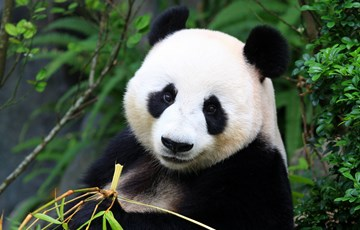
\includegraphics[width=\linewidth]{output/input1.jpg}
        \caption{Input}
        \end{minipage}
        \hfill
        \begin{minipage}{0.4\linewidth}
        \centering
        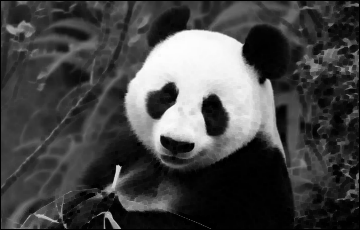
\includegraphics[width=\linewidth]{output/Average Filter_output.png}
        \caption{Output}
        \end{minipage}
        \end{figure}
        \clearpage
        
        \section{Image Scaling}
        \begin{verbatim}
        import sys


input_file = sys.argv[1]
output_file = sys.argv[2]

# Read the input image file line by line
with open(input_file, 'r') as f:
    lines = f.readlines()

# Extract the image dimensions and pixel values
assert lines[0].startswith('P2')
width, height = map(int, lines[2].split())
max_value = int(lines[3])
pixels = [list(map(int, line.split())) for line in lines[4:]]

# Compute the minimum pixel value in the image
min_value = min(min(row) for row in pixels)

# Subtract the minimum value from all pixels
new_pixels = [[p - min_value for p in row] for row in pixels]

# Compute the maximum pixel value in the new image
new_max_value = max(max(row) for row in new_pixels)

# Scale the pixel values in the new image
k = 255  # for 8-bit image
scaled_pixels = [[int(k * p / new_max_value) for p in row] for row in new_pixels]

# Write the processed image to the output file
with open(output_file, 'w') as f:
    f.write('P2\n')
    f.write(f'{width} {height}\n')
    f.write(f'{k}\n')
    for row in scaled_pixels:
        f.write(' '.join(str(p) for p in row))
        f.write('\n')


        \end{verbatim}
        
        \begin{figure}[H]
        \centering
        \begin{minipage}{0.4\linewidth}
        \centering
        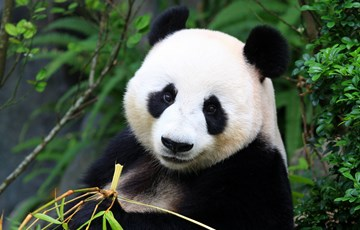
\includegraphics[width=\linewidth]{output/input1.jpg}
        \caption{Input}
        \end{minipage}
        \hfill
        \begin{minipage}{0.4\linewidth}
        \centering
        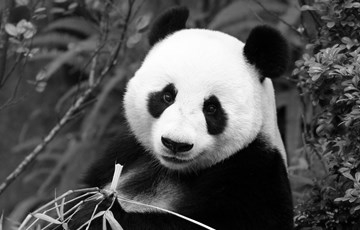
\includegraphics[width=\linewidth]{output/Image Scaling_output.png}
        \caption{Output}
        \end{minipage}
        \end{figure}
        \clearpage
     
\end{document}
